
\chapter{Optimization}

An \textit{optimization problem} has the form

\begin{equation}
    \begin{split}
        minimize &\;\;\;\;\; f_0(x) \\
        subject\;to &\;\;\;\;\; f_i(x) \leq b_i,\;\;\;\;\; i=1, \dots, m.
    \end{split}
\end{equation}


Here the vector $x=(x_1, \dots, x_n)$ is the optimization variable of the problem, the function $f_0~:~\mathbb{R}^n\rightarrow \mathbb{R}$ is the objective function, the functions $f_i~ :~\mathbb{R}^n\rightarrow~\mathbb{R}$, $i=1, \dots, m$, are the (inequality) constraint functions, and the constants $b_1, \dots, b_m$ are the limits, or bounds, for the constraints.

\section{Least-Squares}

A \textit{least-squares} problem is an optimization problem with no constraints and an objective function which is a sum of squares of terms of the form
\begin{equation}
    minimize \;\;\; f_0(x) = ||Ax-b||^2_2
\end{equation}

The solution of such a problem can be reduced to solving a set of linear equations

\begin{equation}
    (A^T A)x=A^Tb,
\end{equation}

which has the following analytical solution: $x = (A^TA)^{-1}A^Tb$.

Some variants exist:
\paragraph{Weighted least-squares} The cost becomes
\begin{equation}
    \sum_{i=1}^{k} w_i(a_i^Tx-b)^2
\end{equation}
which has the following solution: $x=(A^TWA)^{-1}A^TWb$.

\paragraph{Regularized least-squares} The cost is
\begin{equation}
    \sum_ {i=1}^k (a_i^Tx-b)^2 + \rho \sum_{i=1}^n x_i^2,
\end{equation}
Different type of regularizer (the second term) exist and are usually derived form a statistical point-of-view.

\section{Linear Programming}

Another important class of optimization problems is \textit{linear programming}, in which the objective and all constraint functions are linear:

\begin{equation}
    \begin{split}
        minimize &\;\;\;\;\; c^Tx \\
        subject\;to & \;\;\;\;\;a_i^Tx\leq b_i,\;\;\;i=1, \dots,m.
    \end{split}
\end{equation}

There is no analytical formula for the solution of a linear program (as there is for a least-squares problem), but there are a variety of very effective methods. The most famous one is probably the \textbf{simplex algorithm}.

\section{Convex optimization}

A convex optimization problem is one of the form

\begin{equation}
    \begin{split}
        minimize &\;\;\;\;\; f_0(x) \\
        subject\;to &\;\;\;\;\; f_i(x) \leq b_i,\;\;\;\;\; i=1, \dots, m.
    \end{split}
\end{equation}

where the functions $f_0, \dots,f_m : \mathcal{R}^n\rightarrow\mathcal{R}$ are convex, \textit{i.e.}, satisfy
\begin{equation}
    f_i(\alpha x+\beta y)\leq \alpha f_i(x)+\beta f_i(y)
\end{equation}
for all $x,y\in\mathcal{R}^n$ and all $\alpha, \beta \in \mathcal{R}$ with $\alpha+\beta=1$, $\alpha\geq0, \beta\geq0$.

The least-squares problem and the linear programming problem are both special cases of the general convex optimization problem (as convex is a bit more general than linear).

\section{Non-linear optimization}


\subsection{Convexity}


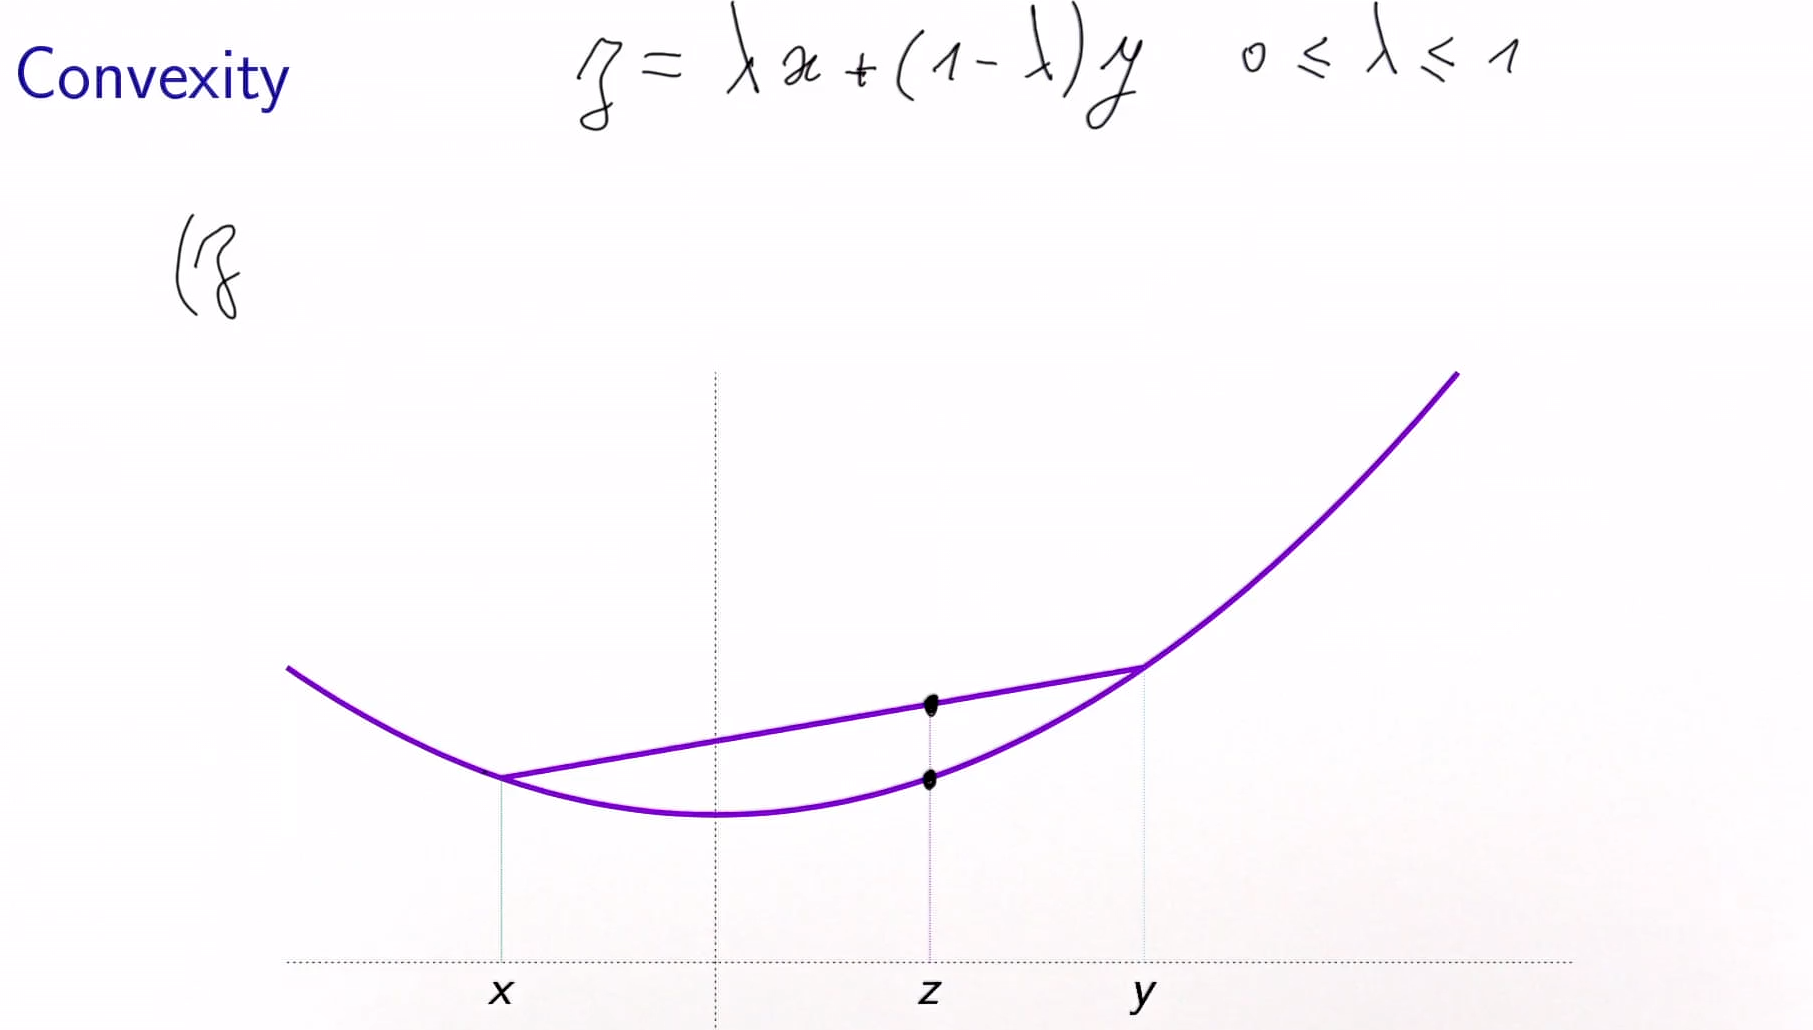
\includegraphics[width=\linewidth]{content/convexity.png}

If the objective function of an optimization problem is convex, it is possible to find a global optimum.

\subsection{First derivative}
The gradient of a function is defined as:

\begin{equation}
    \nabla f(x)=\left(\begin{array}{c}
        \frac{\delta f(x)}{\delta x_1} \\
        \vdots \\
        \frac{\delta f(x)}{\delta x_n}
    \end{array}\right)
\end{equation}

$d$ is a descent direction if $d^T\nabla f(x) < 0$.

For several functions, $f: \mathbb{R}^n\rightarrow\mathbb{R}^m$, the \textbf{Jacobian} matrix is defined as:
\begin{equation}
    J(x) = \left(\begin{array}{c}
        \nabla f_1(x)^T \\
        \vdots  \\
        \nabla f_m(x)^T \\
    \end{array}\right) = \left(\begin{array}{ccc}
        \frac{\delta f_0(x)}{\delta x_0} & \dots & \frac{\delta f_0(x)}{\delta x_n} \\
         \vdots & \ddots & \vdots \\
        \frac{\delta f_m(x)}{\delta x_0} & \dots & \frac{\delta f_m(x)}{\delta x_n} \\
    \end{array}\right)
\end{equation}

The first derivate of a functions describe its slope.



\subsection{Second derivatives}
\begin{equation}
    \nabla f(x): \mathbb{R}^n\rightarrow\mathbb{R}^n
\end{equation}

The gradient matrix of $\nabla f(x)$ is called the \textbf{Hessian} or the second derivatives matrix when it exists:

\begin{equation}
    \nabla(\nabla(f(x))=\nabla^2f(x) \;\; \in \mathbb{R}^n
\end{equation}
The Hessian matrix is symmetric.

\textcolor{red}{If $\nabla^2 f(x)$ is positive semidefinite on $X\subseteq\mathbb{R}^n$, then $f$ is convex on $X$.}


The second derivatives of a function give information about the curvature of the function. The curvature of $f$ in $x$ in direction $d$ is defined as
\begin{equation}
    \frac{d^T\nabla^2 f(x)d}{d^Td}
\end{equation}

\subsection{Linearity and nonlinearity}

A function is linear if it is a linear combination of the parameters:
\begin{equation}
\begin{split}
    f: \mathbb{R}^n \rightarrow \mathbb{R}:&\;\;\; f(x) = \sum_{i=1}^n c_i x_i = c^T x \;\;\; c\in\mathbb{R}^n \\
    f: \mathbb{R}^n \rightarrow \mathbb{R}^m:&\;\;\; f(x) = Ax \;\;\; A\in\mathbb{R}^{m\times n}
\end{split}
\end{equation}

Affine functions are very close
\begin{equation}
\begin{split}
    f(x) = c^T+d \\
    f(x) = Ax+b
\end{split}
\end{equation}

They are usually also included in the term "linear" because the additional constant does not play any role in the optimization.


However, most functions encountered in reality are nonlinear. Actually, a function can have different level of nonlinearity.

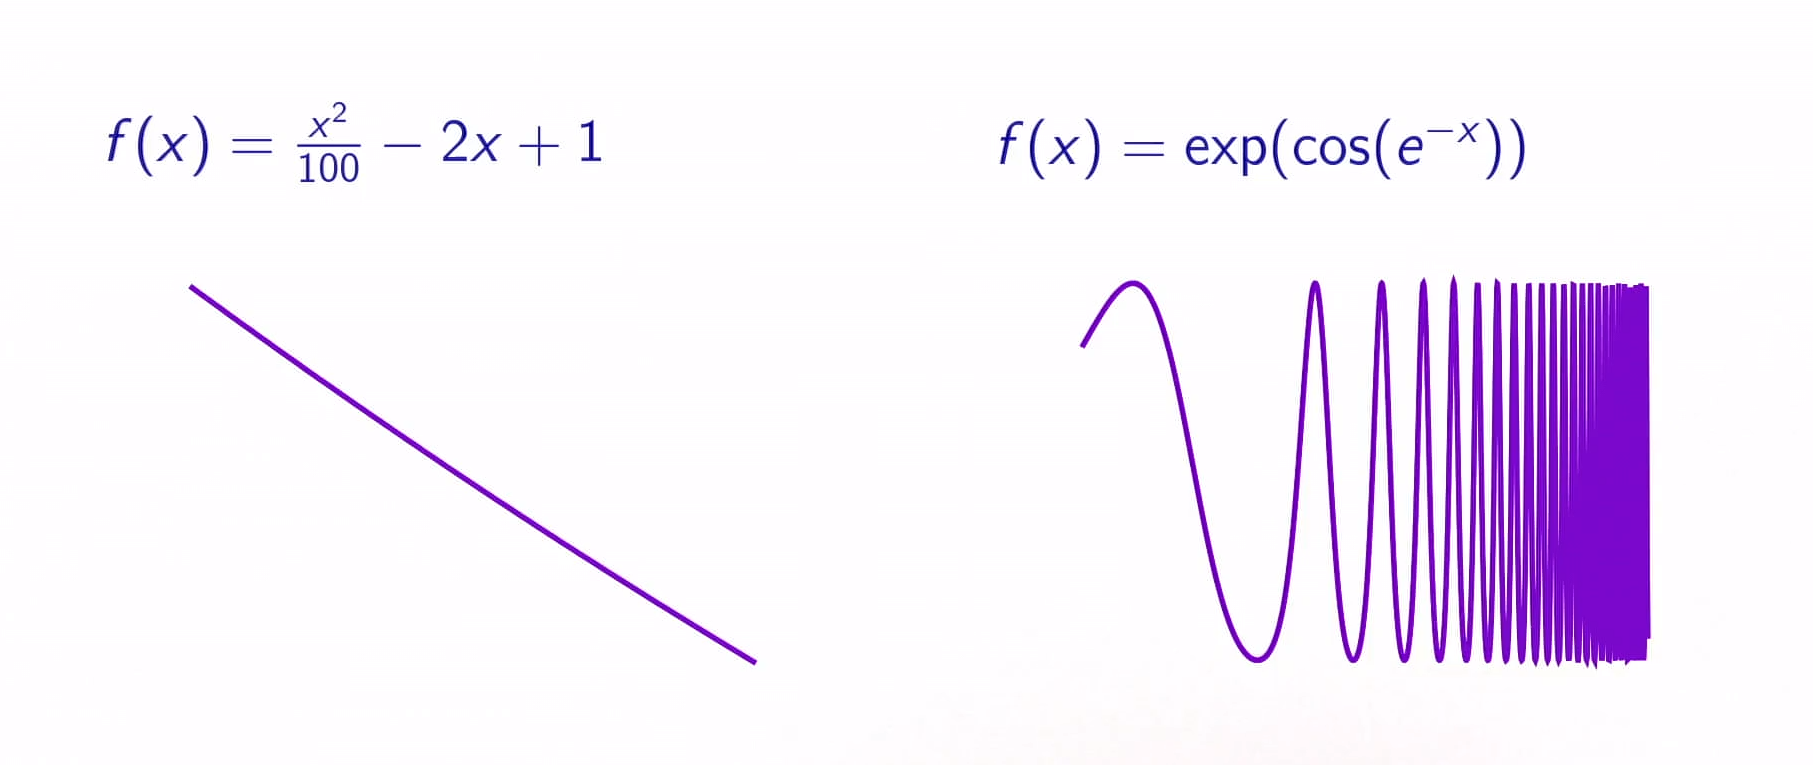
\includegraphics[width=\linewidth]{content/nonlinearity.png}

To characterize if a function is linear or not, we analyze how quickly its derivative is changing. 
The gradient of $f$ is Lipschitz continuous if there exist a $M > 0$ such that, for all $x, y$:
\begin{equation}
    ||\nabla f(x)-\nabla f(y)|| \leq M||x-y||
\end{equation}
M is called the \textbf{Lipschitz constant} of the function.
\begin{itemize}
    \item a small value correspond to almost linear functions
    \item a large value correspond to highly nonlinear functions
\end{itemize}

\subsection{Preconditioning}

The \textbf{condition number} is an indicator of the geometry of a function and its value influences a lot some of the algorithms.
It is possible to change the formulation of the problem in order to get a better value for this indicator. This modification is called \textit{preconditioning}.

\begin{equation}
    k(A) = ||A||\cdot||A^{-1}]||
\end{equation}

and if the matrix $A$ is symmetric positive semidefinite, the condition number is the ratio between the largest and smallest eigenvalues: $k(A) = \frac{\lambda_1}{\lambda_n}$.


For a function with $\nabla^2 f(x)$ positive definite, the eigen value $\lambda_1$ corresponds to the curvature of the function in the direction of its corresponding eigen vector $d_1$. This means that the conditioning number is the ratio between the largest and the smallest curvature.

For example, a 2D function like a valley has a very high curvature in one direction and a small curvature in the orthogonal direction. This means that its condition number is very high, which causes problem during optimization (called ill-conditioned).

The condition number of a function can be modified by a change of variables. Let $M$ be an invertible matrix that defines this change of variable: $x^{\prime}=Mx$ and $x=M^{-1}x^{\prime}$

\begin{equation}
    \begin{split}
        \tilde{f}(x^{\prime}) & = f(M^{-1}x^{\prime}) \\
        \nabla\tilde{f}(x^{\prime}) & = M^{-T}\nabla f(M^{-1}x^{\prime}) \\
        \nabla^2\tilde{f}(x^{\prime}) & = M^{-T}\nabla^2 f(M^{-1}x^{\prime})M^{-1} \\
        & = M^{-T}\nabla^2 f(x)M^{-1}
    \end{split}
\end{equation}


\subsection{Necessary optimality conditions}

$x^*$ is a local minimum of $f:\mathbb{R}^n \rightarrow\mathbb{R}$.

If $f$ is differentiable around $x^*$, then
\begin{equation}
    \nabla f(x^*)=0
\end{equation}

If $f$ is twice differentiable around $x^*$, then

\begin{equation}
    \nabla^2f(x^*) \geq 0 \;\;\;\; [positive\;semidefinite]
\end{equation}

These conditions are necessary but not sufficient.

Also, because the second derivative is positive semidefinite, it means that the function is locally convex around $x^*$.
All the eigenvalues of the Hessian are non-negative ($\geq 0$) and, as they represent the local curvature of the function, it means that the function is locally convex.

\subsection{Sufficient optimality conditions}

Consider $x^*$ and $f : \mathbb{R}^n \rightarrow \mathbb{R}$ twice differentiable,
If

\begin{equation}
    \nabla f(x^*) = 0
\end{equation}

and
\begin{equation}
    \nabla^2 f(x^*) > 0 \;\;\;\;[positive\;definite]
\end{equation}

then $x^*$ is a local minimum.


\textcolor{red}{These conditions apply only to local minima, but we cannot be sure that it is a global optimum.}


\paragraph{Condition for global minimum}

$x^*$, a local minimum of $f$, is also a global minimum if $f$ is convex (not just locally).
$x^*$, is the unique global minimum if $f$ is strictly convex.


\subsection{Quadratic functions}
The second derivative of a quadratic function is constant.

\begin{equation}
    f(x) = \frac{1}{2} x^T Q x + g^Tx + c
\end{equation}
where $Q\in \mathbb{R}^{n\times n}$ is symmetric, $g\in \mathbb{R}^n$ and $c\in \mathbb{R}$.

\begin{itemize}
\item It is always possible to write $Q$ as a symmetric matrix, so no loss of generality.
\item The $\frac{1}{2}$ factor is just added to simplify the calculation of the derivative.
\end{itemize}


\begin{equation}
    \begin{split}
        &\nabla f(x) = Qx+g \\
        &\nabla^2 f(x) = Q
    \end{split}
\end{equation}

\paragraph{Case $Q < 0$:}
If $Q$ is not positive semidefinite, it means that at least one eigen value is negative. Thus, there exist a direction along which the function is concave and thus the result is unbounded.

\paragraph{Case $Q > 0$:}
If $Q$ is \textbf{positive definite}, all eigenvalues are strictly positive and the problem is strictly convex. The unique global minimum is obtained by solving
\begin{equation}
    \nabla f(x^*) = 0 \iff Qx^* + g = 0
\end{equation}

\paragraph{Case $Q \geq 0$ but $Q \not> 0$:} All eigenvalues are positive but some of them are zero. This means that the function has a 0 curvature in some direction, thus is linear in some directions.
\begin{itemize}
    \item Call $K$ the subspace spanned by the eigenvectors with positive eigenvalues.
    \item Call $N$ the subspace spanned by the eigenvectors with zero eigenvalues.
    \item The function is strictly convex in $K$.
    \item The function is linear in $N$.
    \item Depending on the linear part, the problem is either unbounded (slope of linear part $\neq 0$) or there are an infinite number of solutions (the linear part is flat).
\end{itemize}

\section{Newton's method}
\subsection{Solving equations}
Optimization algorithms heavily rely on solving the system of equations that are defined by the optimality equations.
\begin{itemize}
    \item If the system is linear, we can use Gaussian elimination.
    \item If the system is nonlinear, we need to use Newton's method.
\end{itemize}

\subsubsection{Newton's method (root finding)}
\paragraph{One variable function:}
The method start at an initial point, calculate the tangent, solve the equation for this tangent (where does the line intersect the x-axis) and repeat.

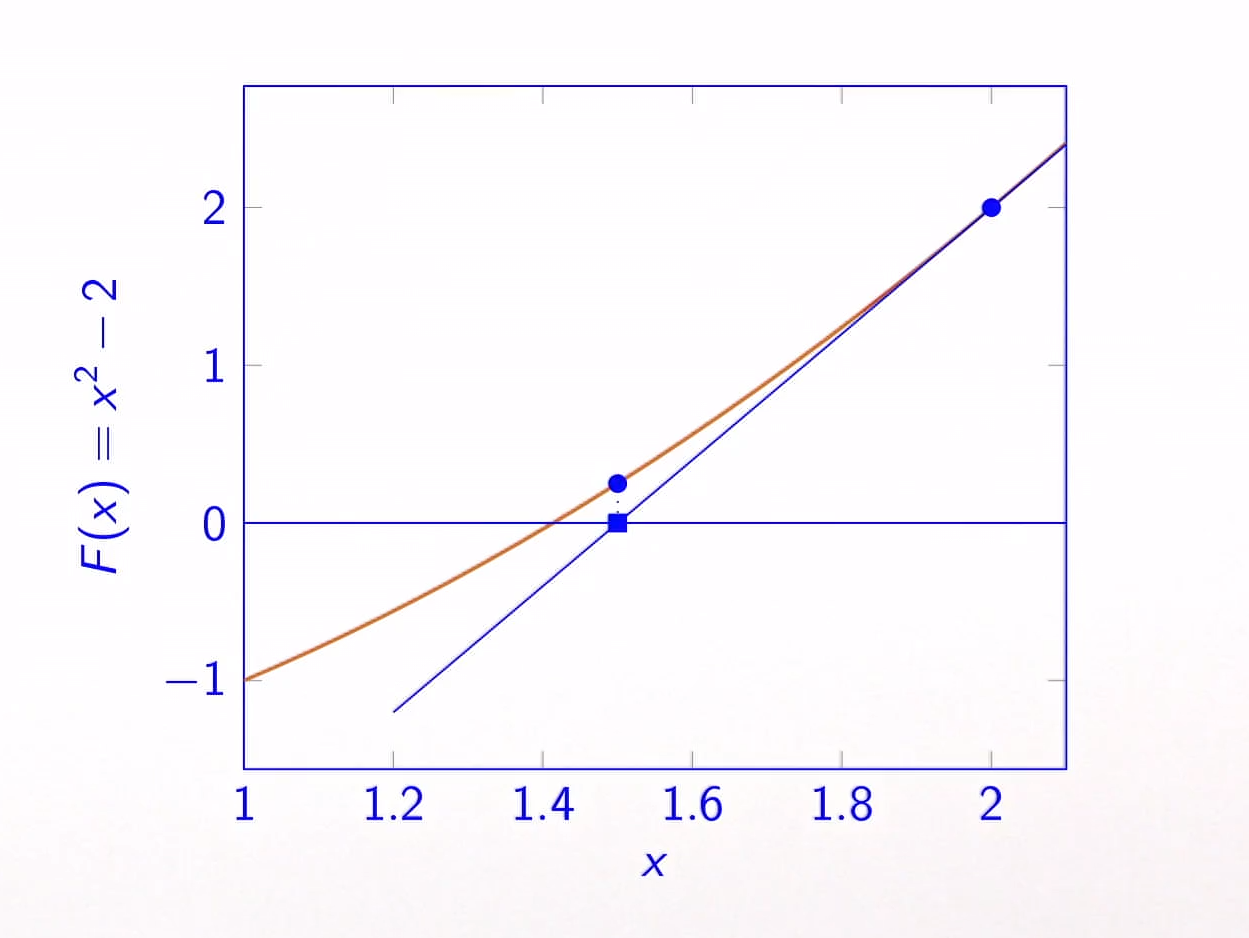
\includegraphics[width=\linewidth]{content/newton_root_finding.png}


The method is very fast, quadratically convergence (the precision doubles at each iteration).

We use the tangent approximation (model) at $\hat{x}$.

\begin{equation}
    m_{\hat{x}}(x)=F(\hat{x}) + (x-\hat{x}) F^{\prime}(\hat{x})
\end{equation}

At each iteration, find $x_{k+1}$ that solves
\begin{equation}
    m_{x_k}(x) = F(x_k) + (x-x_k)F^{\prime}(x_k) = 0
\end{equation}

\begin{equation}
    \begin{split}
        F(x_k)+(x_{k+1}-x_k)F^{\prime}(x_k) &= 0 \\
        (x_{k+1}-x_k)F^{\prime}(x_k) &= -F(x_k) \\
        (x_{k+1}-x_k) &= -F(x_k) / F^{\prime}(x_k) \\
        x_{k+1} &= x_k - F(x_k) / F^{\prime}(x_k)
    \end{split}
\end{equation}

The solution is defined only if the $F^{\prime} \neq 0$.
Convergence is not always guaranteed. There are three conditions to guarantee the convergence:
\begin{enumerate}
\item F is not too nonlinear. $F^{\prime}$ is Lipschitz continuous (its Lipschitz constant $M$ is no too large).
\item $F^{\prime}$ is not too close to 0 (because of the division): $\exists \rho>0$ such that $|F^{\prime}(x)| \geq \rho,\;\forall x$.
\item $x_0$ is not too far from the solution: $\exists \eta>0$ such that $|x_0-x^*| < \eta$.
\end{enumerate}
If these three conditions are met, Newton's method is well defined (no problem with the division) and it converges \textit{q-quadratically} towards $x^*$.
\begin{equation}
    |x_{k+1}-x^*| \leq \frac{M}{2\rho} |x_{k}-x^*|^2
\end{equation}
The speed of convergence will change with $M$ (the Lipschitz constant) and $\rho$. When $M$ is small (almost linear function) the convergence is fast. When $\rho$ is large (derivative far from 0) the convergence is fast.
\paragraph{Multiple variables}


\begin{equation}
\begin{split}
    m_{\hat{x}} &= F(\hat{x}) + \nabla F(\hat{x})^T (x-\hat{x}) \\
    &= F(\hat{x}) + J(\hat{x})(\hat{x})^T (x-\hat{x})
\end{split}
\end{equation}

The iteration becomes
\begin{equation}
    x_{k+1}=x_k+d_k    
\end{equation}
where $d_k$ should satisfy the equation
\begin{equation}
    \begin{split}
        J(x_k)d_k & = -F(x_k) \\
        d_k & = -J(x_k)^{-1}F(x_k)
    \end{split}
\end{equation}

    


\subsection{Newton's local method}
The algorithm is motivated by the necessary condition for optimality: $\nabla f(x) = 0$. This gives a system of $n$ equations, that can be solved with the Newton's method (for root finding).

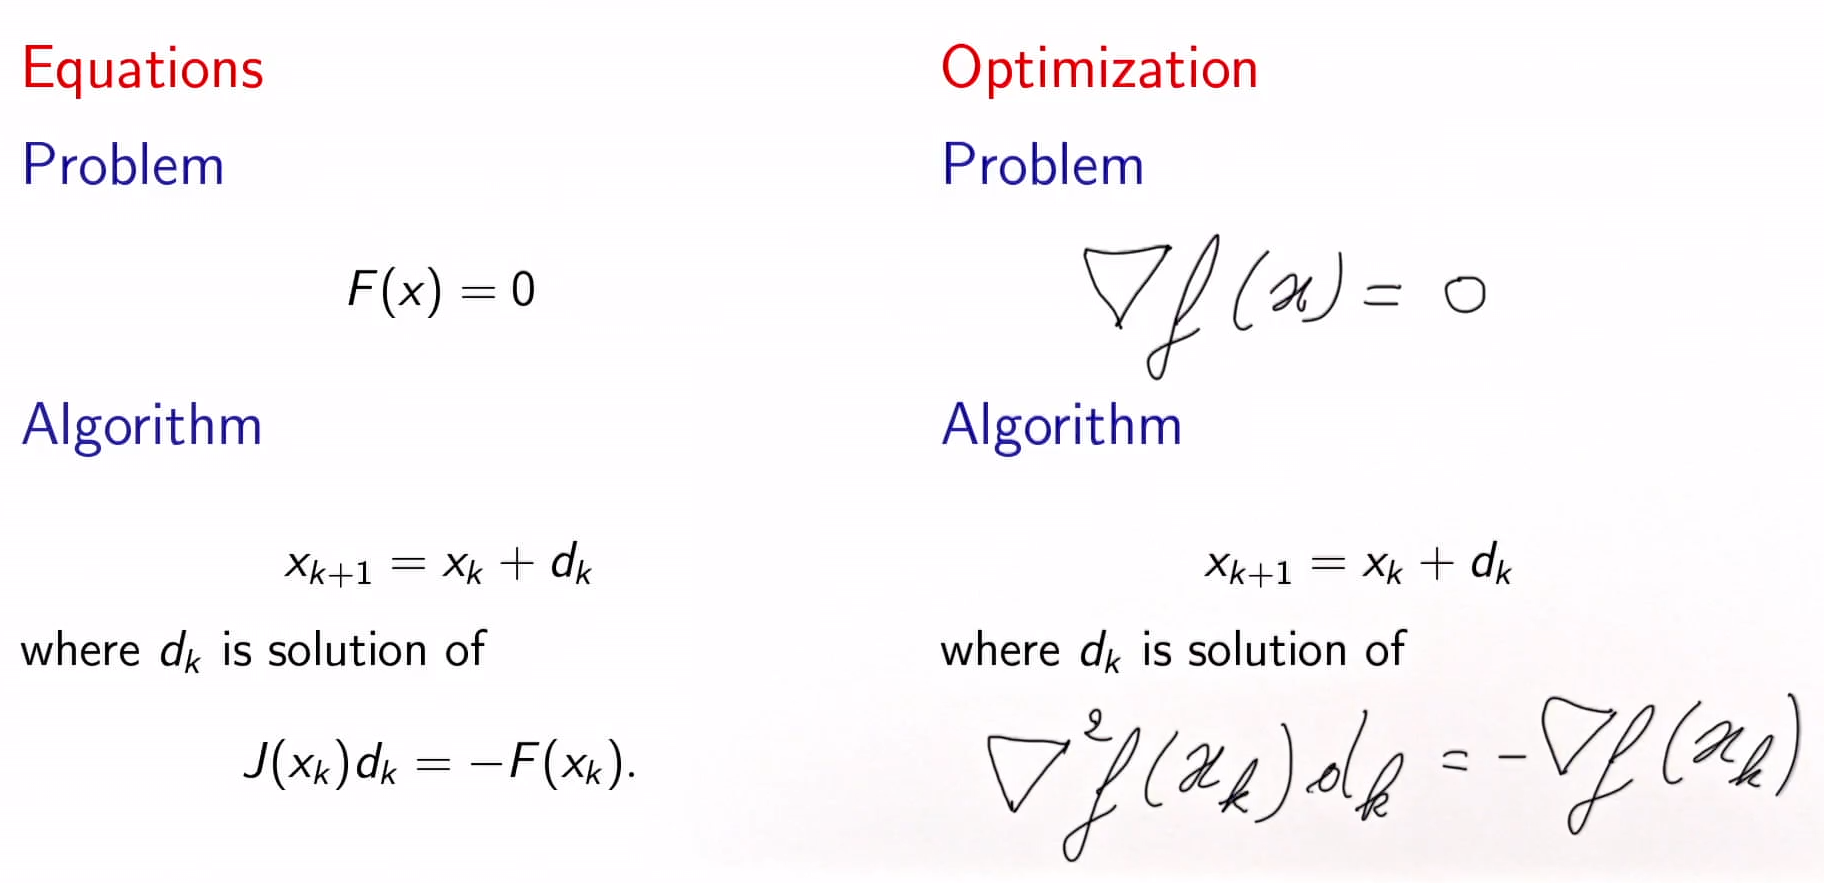
\includegraphics[width=\linewidth]{content/Newton_optimization.png}

Newton's method for solving equations does not always work, but when it does work it is very fast.
Even if it converges towards a point where $\nabla f(x) = 0$, we need to check the second derivative is positive definite. If the eigenvalues of the Hessian matrix are both positive and negative, the results is a saddle point, which is not a local minimum.

\paragraph{Geometric interpretation}

The Newton's method for solving a system of equations uses a linear approximation of the function (the tangent). In the case of optimization, the we use a quadratic model.

\begin{equation}
    m_{\hat{x}}(x)=f(\hat{x}) + (x-\hat{x})^T \nabla f(\hat{x}) + \frac{1}{2}(x-\hat{x})^T \nabla^2 f(\hat{x}) (x-\hat{x})
\end{equation}

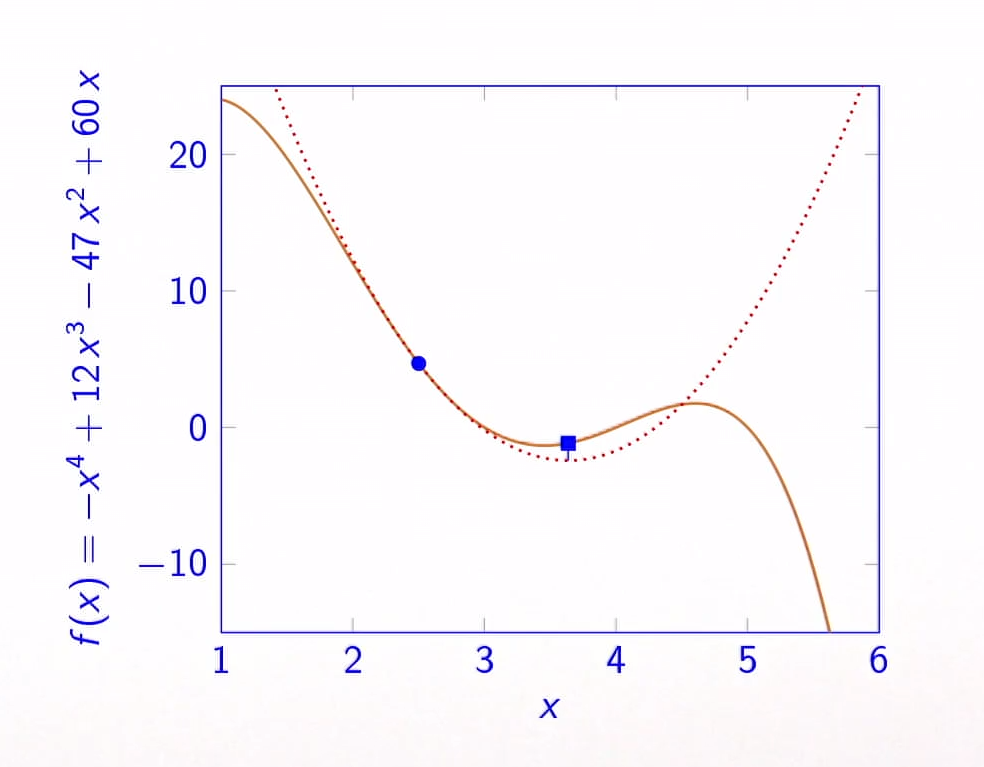
\includegraphics[width=\linewidth]{content/newton_quadratic_model.png}

The idea is to minimize the quadratic model (parabola) instead of the function.

Three cases can happen:
\begin{itemize}
    \item The function is convex around the current point, the method converges well.
    \item The function is convex around the current point, but it does not match at all the function around the optimum. Therefore it may generate points that are worse.
    \item The function is concave around the current point, and thus, the quadratic model is concave and cannot be minimized.
\end{itemize}

\paragraph{Newton's point} It is the point that is obtained after applying one iteration of local Newton's method to a current iterate $x_k$.
It is defined when $\nabla^2 f(x_k) > 0$ by

\begin{equation}
    x_N = x_k + d_N
\end{equation}

where $d_N$ verifies the Newton's equations:
\begin{equation}
    \nabla^2 f(x_k) d_N = -\nabla f(x_k)
\end{equation}

\paragraph{Cauchy's point} It is another interesting point, which is defined as the minimum point of the quadratic model in the direction of minus the gradient. 

It is defined when the model is convex in the direction of the gradient ($\nabla f(x_k)^T \nabla^2 f(x_k) \nabla f(x_k)~>~0$) by:

\begin{equation}
    x_C = x_k - \alpha_C \nabla f(x_k)
\end{equation}
where 
\begin{equation}
    \alpha_C = \frac{\nabla f(x_k)^T\nabla f(x_k)}{\nabla f(x_k)^T\nabla^2 f(x_k) \nabla f(x_k)}
\end{equation}

\paragraph{Conclusion} Newton's method for optimization is based using a quadratic model to locally approximate the function and choosing the minimum of this model for the next iteration. However, there are two major problems:
\begin{itemize}
    \item The quadratic model might be a poor approximation of the function at the optimum point, which can generate results that are worse in terms of objective functions.
    \item If the function is locally concave at the current point, the model will be concave and cannot be minimized.
\end{itemize}


\section{Descent methods}


With descent, we first find a descent direction and then calculate how far we should go (the step size).
The most natural direction is \textbf{minus the gradient}, because it is the steepest direction (the direction in which the function decreases the fastest). At each iterate we stop at the Cauchy's point. The problem is that the convergence is \textbf{very slow} ("zig-zag" behaviour).


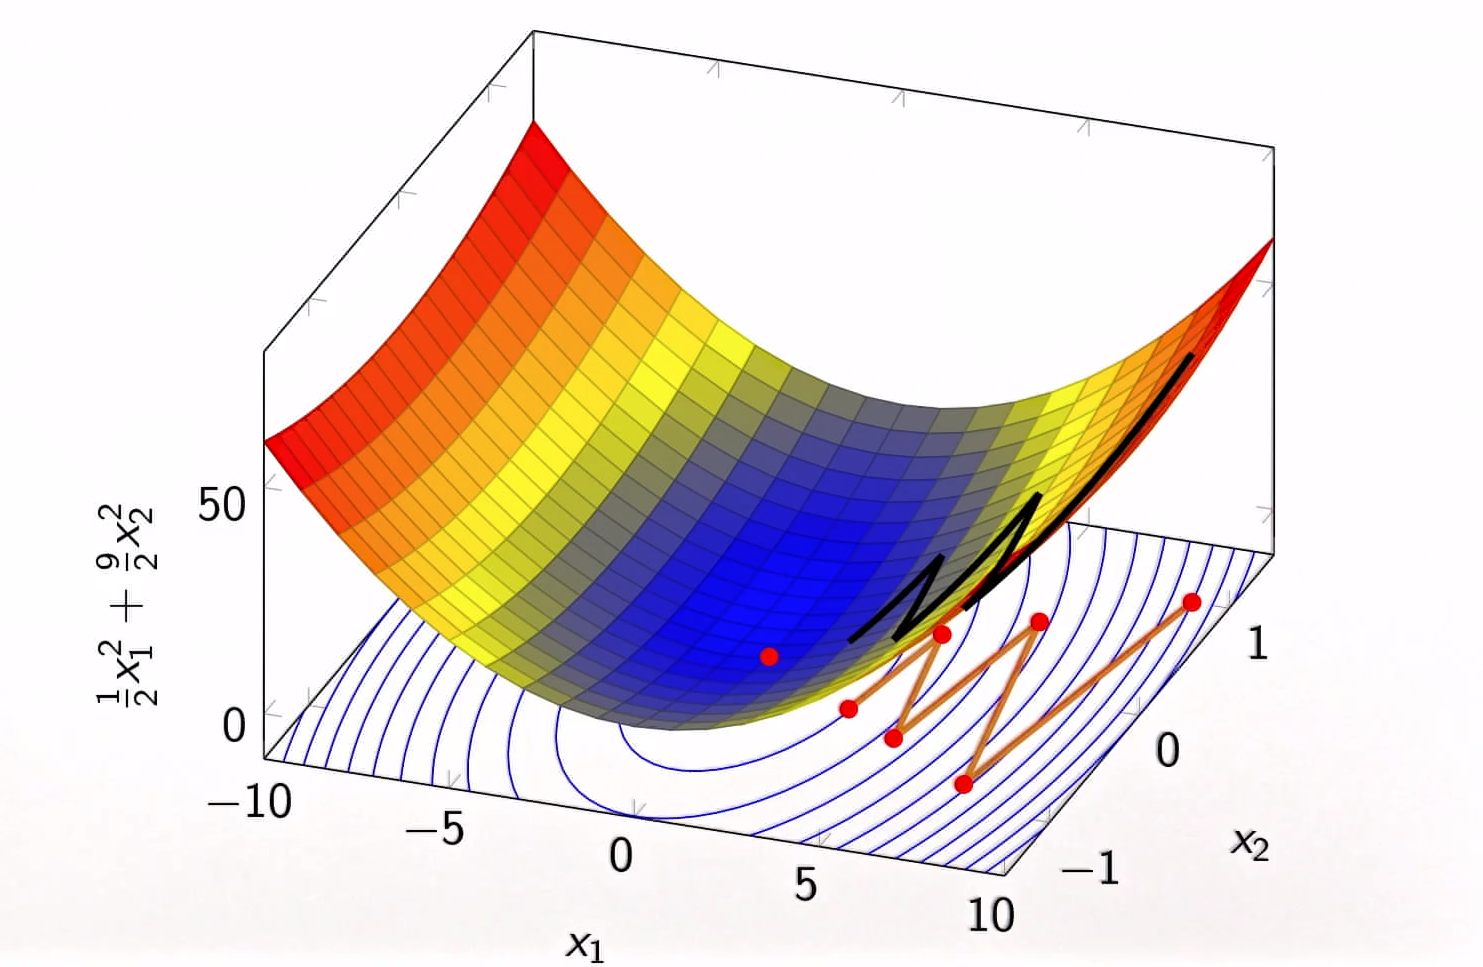
\includegraphics[width=\linewidth]{content/steepest_descent_problems.png}

\textbf{Preconditionning} (a change of variables) can help a lot (1 step-convergence instead of 55 steps). Let $H_k$ a symmetric positive definite matrix. We can compute its Cholesky decomposition: $H_k=L_kL_k^T$ and select $L_k^T$ as defining the change of variable.
The change of variable is:
\begin{equation}
    x^{\prime} = L_k^T x
\end{equation}

Steepest descent direction:
\begin{equation}
    x^{\prime}_{k+1} = x^{\prime}_ k - \alpha_k \nabla \tilde{f}(x^{\prime}_k)
\end{equation}


\begin{equation}
    \begin{split}
        \tilde{f}(x^\prime) =& f(L_k^{-T}x^\prime) \\
        \nabla \tilde{f}(x^\prime) &= L^{-1}_k \nabla f(L_k^{-T}x^\prime) \\
    \end{split}
\end{equation}

The descent step becomes:
\begin{equation}
    x_{k+1}^\prime = x_k^\prime - \alpha_k L_k^{-1} \nabla f(L_k^{-T}x_k^\prime)
\end{equation}

Going back to the original variable $x$, we finally get:
\begin{equation}
    x_{k+1} = x_k - \alpha_k H_k^{-1} \nabla f(x_k)
\end{equation}

This equation combines the change of variables, apply the steepest descent on that variable and come back to the original variable.
It is guaranteed that this direction $-H_k^{-1}\nabla f(x_k)$ is a descent direction.

\paragraph{Exact line search}: Some other methods exists:
\begin{itemize}
    \item Quadratic interpolation: Choose 3 points $a < b < c$ such that $f(b) < f(a)$ and $f(b) < f(c)$, then fit a parabola to these three points, update $a, b, c$ and repeat.
    \item Golden Section: see course.
\end{itemize}